\graphicspath{{3exp/asy/}}

\section{Exponential and Logarithmic Functions \& Models}

Introducing exponential functions without calculus presents a significant challenge. The simplest approach is as a short-hand notation for \emph{repeated multiplication}: for instance
\[
	a^5=a\cdot a\cdot a\cdot a\cdot a
\]
analogous to how multiplication represents repeated addition
\[
	5a=a+a+a+a+a
\]
The problem with this approach is that it doesn't help you understand what should be meant by, say, $a^{3/4}$ or $a^{\sqrt 2}$: multiplying something by itself `$\sqrt 2$ times' sounds\footnote{The same issue arises for multiplication: $3\sqrt 2=\sqrt 2+\sqrt 2+\sqrt 2$ is relatively easy to understand, but how would you convince someone what $\pi\sqrt 2$ means?} insane!\smallbreak
To rigorously address this problem requires \emph{continuity} and other ideas surrounding the foundations of calculus which you'll encounter in upper-division analysis; topics unsuitable for this course. Instead, we assume some familiarity with exponential functions via introductory calculus, where they are unavoidable and offer two ways to introduce exponential functions and $e$ via modelling.


\subsection{The Natural Growth Model}

A basic model for any variable quantity is that its \emph{rate of change be proportional to the quantity itself.} This idea necessarily needs some calculus; as a differential equation,
\[
	\diff[y]{x}=ky
\]
where $k$ is a constant; if $k>0$ this is the \emph{natural growth equation}, if $k<0$ the \emph{natural decay equation.} This is commonly encountered when modelling \emph{population growth}; an otherwise unconstrained population seems like its growth rate should be proportional to its size (twice the people, twice the babies\ldots). This model is hugely applicable, since \emph{population} can refer to essentially any quantifiable value: people, bacteria, money, reagents in a chemical/nuclear reaction, etc.


\begin{example}[lower separated=false, sidebyside, sidebyside align=top seam, sidebyside gap=0pt, righthand width=0.28\linewidth]{}{naturalgrowth}
	The simplest natural growth equation has $k=1$:
	\[
		\diff[y]{x}=y
	\]
	If a point $(x,y)$ lies on a \textcolor{Green}{solution curve,} then the differential equation tells us the \emph{direction of travel} of the solution. We may visualize this by drawing an arrow with \text{slope} $\diff[y]{x}=y$; the arrows are \emph{tangent} to any solution.\footnotemark{} You should easily be able to sketch some other solution curves.\smallbreak
	You should, of course, recognize the graph\ldots
	\tcblower
	\flushright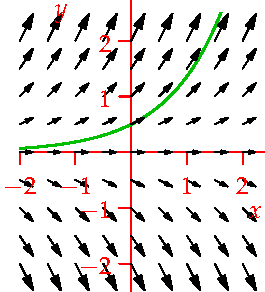
\includegraphics[scale=1]{slopefields-01}
\end{example}

\footnotetext{A similar approach is available for any first-order differential equation $\diff[y]{x}=F(x,y)$: the equation defines its \emph{slope field} (arrows), to which  solution curves must be tangent.}


\begin{defn}{}{}
	Let $a>0$ be constant. The \emph{exponential function with base $a$} is $f(x)=a^x$.
\end{defn}

Recall the \emph{exponential laws,}\phantomsection\label{pg:explaws} which are very natural when $x,y,r$ are positive integers:
\[
	\tcbhighmath{a^{x+y}=a^xa^y\qquad a^{x-y}=\frac{a^x}{a^y}\qquad (a^x)^r=a^{rx}}
\]
These hold for all exponents, with the same continuity caveats we saw previously. 
For modelling, the crucial property of exponential functions is that they have proportional derivative.

\begin{thm}{}{}
	The rate of change of $f(x)=a^x$ is proportional to $f(x)$. Specifically,
	\[
		f'(x)=\lim_{h\to 0}\frac{a^{x+h}-a^x}h=a^x\lim_{h\to 0}\frac{a^{h}-1}h
	\]
	so that $f(x)=a^x$ satisfies the natural growth/decay equation $\diff[y]{x}=ky$ with proportionality constant
	\[
		k=f'(0)=\lim_{h\to 0}\frac{a^{h}-1}h
	\]
\end{thm}

\goodbreak


\begin{example}{}{}
	We estimate the proportionality constant $\displaystyle k=\smash[b]{\lim\limits_{h\to 0}\frac{a^{h}-1}h}$ to 3\,d.p.\ using a calculator for four values of $h$:
	\[
		\def\arraystretch{1.5}
		\begin{array}{c|cccccc}
			a&2&2.5&2.7&2.75&3&5\\\hline\hline
			\frac{a^{0.1}-1}{0.1}&0.718&0.960&1.044&1.065&1.161&1.746\\\hline
			\frac{a^{0.01}-1}{0.01}&0.696&0.921&0.998&1.017&1.105&1.622\\\hline
			\frac{a^{0.001}-1}{0.001}&0.693&0.917&0.994&1.012&1.099&1.611\\\hline
			\frac{a^{0.0001}-1}{0.0001}&0.693&0.916&0.993&1.012&1.099&1.610
			%\frac{a^{0.01}-1}{0.01}&0.696&&&&&\\\hline
			%\frac{a^{0.001}-1}{0.001}&0.693&&&&&
		\end{array}
	\]
	What is happening to the proportionality constant as $a$ increases? As $h$ decreases?
\end{example}

It appears as if there is a special number somewhere between 2.7 and 2.75 for which the proportionality constant is precisely $k=1$.





\begin{defn}{}{}
	The value $e=2.71828\ldots$ is the unique real number such that $\smash[b]{\lim\limits_{h\to 0}\frac{e^h-1}h =1}$.\smallbreak
	The \emph{natural\footnotemark{} exponential function} $\exp(x)=e^x$ has derivative $\diff xe^x=e^x$.
\end{defn}

\footnotetext{\emph{Natural} here means \emph{unavoidable}: an old cliche suggests that if aliens were to land on Earth, they'd have to understand $e$ given the technology they'd require to get here. Of course they'd likely use a different symbol; ours comes from Leonhard Euler around 1728. Like $\pi$ and $\sqrt 2$, the constant $e$ is an \emph{irrational number}: its decimal representation contains no repeating pattern. There isn't the same geeky fascination with memorizing the digits of $e$ as there is with $\pi$, neither is there an `$e$-day' (Feb 7\th{} at 6:28\,p.m.\ anyone?).}

The function $f(x)=\frac 12e^x$ is plotted in Example \ref{ex:naturalgrowth}. Of course there are many other solutions to the natural growth equation $\smash{\diff[y]{x}=y}$: for any constants $c,k$,
\[
	y=ce^{kx}\implies\diff[y]{x}=\diff x ce^{kx}=cke^{kx} = ky
\]
In fact the converse also holds; for the details, take a differential equations course!

\begin{thm}{}{natgrowth}
	The solutions to the natural growth equation $\diff[y]{x}=ky$ are precisely the functions
	\[
		y(x)=y_0e^{kx} =y_0\exp(kx)
	\]
	where $y_0=y(0)$ is the initial value.
\end{thm}



\begin{example}{}{}
	A Petri dish contains a population $P(t)$ of bacteria satisfying the natural growth equation $\diff[P]{t}=0.5P$ where time is measured in weeks from the start of the year.\par
	\begin{minipage}[t]{0.63\linewidth}\vspace{-2pt}
		If $P(0)=100$ bacteria, then $P(t)=100e^{0.5t}$. Specifically, at the end of January ($4\frac 37$ weeks) one expects there to be
		\[
			P(\tfrac{31}7)=100\exp\tfrac{31}{14}=915\text{ bacteria}
		\]
		Note that the exponential doesn't return 915 exactly; this is only an approximation. Models like this work best for large populations where integer rounding errors are of minimal concern.
	\end{minipage}
	\hfill
	\begin{minipage}[t]{0.35\linewidth}\vspace{-5pt}
		\flushright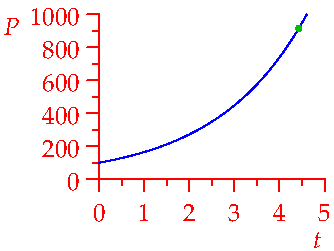
\includegraphics{bacteria}
	\end{minipage}
\end{example}


\boldsubsubsection{Compound Interest and the Discovery of $e$}

The first description of $e$ came in 1683 when Jacob Bernoulli tried to model the growth of money in a hypothetical bank account. We give a modernized version of his approach.

\begin{example}{}{}
	\$1 is deposited in an account paying 100\% interest per year (nice!). Bernoulli observed that the money in the account at the end of the year depends on \emph{when} the interest is paid.
	\begin{itemize}
	  \item If the interest is paid once at the end of the year (this is called \emph{simple} interest), you'll have \$2.
	  \item If half the interest (50\textcent) is paid at six months, then the balance (\$1.50) earns $\frac 12\cdot 1.50=75$\textcent\ interest for the rest of the year; you'll finish the year with \$2.25 in the account.
	  \item If the interest is paid in four installments, we have the following table of transactions (data is rounded to the nearest cent)
	  \begin{quote}
		  \begin{tabular}{c|c|c}
			  Date&Interest Paid&Balance\\\hline\hline
			  1\st\ Jan&---&\$1\\\hline
			  1\st\ Apr&25\textcent&\$1.25\\\hline
			  1\st\ July&$\frac 14\cdot 1.25=31$\textcent&\$1.56\\\hline
			  1\st\ Oct&$\frac 14\cdot 1.56=39$\textcent&\$1.95\\\hline
			  New Year&$\frac 14\cdot 1.95=49$\textcent&\$2.44
		  \end{tabular}
	  \end{quote}
	  More succinctly, the year-end balance is $\left(1+\frac 14\right)^4=$ \textdollar 2.44.
	  \goodbreak
	  
	  \item More generally, if the interest is paid over $n$ equally spaced intervals, the account balance at the end of the year would be \textdollar$\left(1+\frac 1n\right)^n$. Here are a few examples rounded things to 5\,d.p.
	  \begin{quote}
	  	\def\arraystretch{1.5}
		  \begin{tabular}{l|l}
			  Frequency&Balance after 1 year (\textdollar)\\\hline\hline
			  Every month&$\left(1+\frac 1{12}\right)^{12}=2.61304$\\\hline
			  Every day&$\left(1+\frac 1{365}\right)^{365}=2.71457$\\\hline
			  Every hour&$\left(1+\frac 1{8760}\right)^{8760}=2.71813$\\\hline
			  Every second&$\left(1+\frac 1{31536000}\right)^{31536000}=2.71828$
		  \end{tabular}
	  \end{quote}
	 	As the frequency of payment increases, it appears as if the balance is increasing to \textdollar$e$\ldots
	\end{itemize}
\end{example}


In fact this is a theorem, though it requires significant work (beyond this class) to prove it:
\[
	\tcbhighmath{e=\lim_{n\to\infty}\left(1+\frac 1n\right)^n\quad\text{and more generally}\quad e^x =\lim_{n\to\infty}\left(1+\frac xn\right)^n}
\]
This again shows that $e$ arises very naturally.

\boldinline{Simple, Monthly \& Continuous Interest}

In finance, interest is typically computed in one of three ways. In each case we describe the result of investing \$1 at an annual interest rate of $r\%=\frac r{100}$.
\begin{description}
	\item[\normalfont\emph{Simple interest}] You are paid $\frac r{100}$ dollars at the end of the year. Your invested dollar becomes $1+\frac r{100}$ dollars.
	\item[\normalfont\emph{Monthly interest}] Each month you are paid $\frac r{12}$\% of your current balance. This amounts to a balance of $(1+\frac r{1200})^{12}$ dollars at year's end. The period need not be monthly: if interest is paid in $n$ installments, the balance would be $(1+\frac r{100n})^{n}$.
	\item[\normalfont\emph{Continuous interest}] After $t$ years (can be any fraction of a year!) your dollar-balance is
	\[
		e^{\frac{rt}{100}}=\exp\frac{rt}{100} =\lim_{n\to\infty}\left(1+\frac{rt}{100n}\right)^n
	\]
\end{description}

\begin{example}{}{}
	A bank account earns 6\% annual interest paid monthly. To what simple annual interest rate does this correspond? Would you perfer an account paying 6\% continuously?\smallbreak
	At the end of the year, \$1 becomes
	\[
	 	\left(1+{0.06}{12}\right)^{12}=1.005^{12}\approx 1.06168\ldots
	\]
	corresponding to a simple interest rate of 6.17\%. By cobntrast, 6\% continuous interest would result in your dollar becoming $e^{6/100}\approx 1.06184$, corresponding to a (marginally) higher simple interest rate of 6.18\%. You should prefer this, particularly if you have a lot of money to invest! The difference is more noticable with an investment of \$1000 over ten years:
	\[
		1000\times 1.005^{120}=\$1819.40
		\quad\text{versus}\quad
		1000e^{0.6}=\$1822.12
	\]
\end{example}

\goodbreak

There are several reasons for these varying approaches, not all of them consumer-friendly:
\begin{enumerate}\itemsep0pt
  \item Simple interest is simple! It is easy to understand and compute, but hard to decide how or even whether to compute interest for parts of a year.
  \item Monthly interest fits with most paychecks, so is sensible for loans, particularly mortgages.
  \item Continuous interest allows the balance of an account to be found easily at any time, even between interest payment dates. It is also much easier to apply mathematical analysis (calculus).
  \item A company can make an interest rate appear \emph{higher} (if a savings account) or \emph{lower} (if a loan) by choosing which way to quote an interest rate.
\end{enumerate}


\begin{example}{}{}
	A bank quotes you a loan with a continuously compounded interest rate of 7\%. If you borrow \textdollar 100,000, then at the end of the year you'll owe
		\[
			100000e^{0.07} =\$107,250.82
		\]
		not the \$107,000 you might have expected! This corresponds to a simple interest rate (one payment at the end of the year) of 7.25\%.\footnotemark{}
\end{example}

\footnotetext{In the US, mortgage companies typically quote an interest rate which they use to compound \emph{monthly.} For example, if the quoted rate is 7\%,
  then the effective annual (simple) interest rate is $\left(1+\frac{0.07}{12}\right)^{12}-1=7.229\%$.
  By law, this higher \emph{effective APR} must be quoted somewhere, though it is unlikely to be as prominently posted\ldots}



\begin{exercises}{}{}
\exstart Draw a slope field for the natural decay equation $\diff[y]{x}=-\frac 13y$ and use it to sketch the solution curve with initial condition $y(0)=6$. What is the \emph{function} $y(x)$ in this case?

\begin{enumerate}\setcounter{enumi}{1}
  \item Which of the following would you prefer for a savings account? Why?
	\begin{itemize}
  	\item 5\% interest paid continuously. %5.127
  	\item 5.05\% compounded monthly. %5.168
  	\item 5.1\% paid at the end of the year. 
	\end{itemize}
	
   
  \item You invest \$1000 in an account that pays 4\% simple interest per year.
  \begin{enumerate}
    \item How much money will you have after 5 years?
    %\item To what \emph{continuous} rate of interest is 4\% equivalent?
    \item If you close the account after 2 years and 3 months, the bank needs to decide how much interest to credit you with. Do this is two ways (the answers will be different!):
    \begin{enumerate}
      \item Compute using the simple interest rate for 2.25 years ($(1+\frac r{100})^{2.25}$).
      \item Suppose that interest is paid at 4\% for all completed years and then at 4\% paid monthly for any completed months of an incomplete year. Find the balance of the account at closing.
    \end{enumerate}
	\end{enumerate}


  \item See if you can explain why the proportionality constant for $\left(\frac 1a\right)^x$ is \emph{negative} that for $a^x$: that is,
  \[
  	\lim_{h\to 0}\frac{(\frac 1a)^h-1}h=-\lim_{h\to 0}\frac{a^h-1}h
  \]
  Try to find both an \emph{algebraic} reason and a \emph{pictorial} one.
  
  \item Sketch the function $f(x)=e^{-x^2}$. Where have you seen this before, and what uses does this function have?
\end{enumerate}
\end{exercises}


\clearpage



\subsection{Logarithmic Functions}

Since $e>1>0$, the exponential satisfies the following properties:
\[\lim_{x\to-\infty}e^x=0,\qquad \lim_{x\to\infty}e^x=\infty,\qquad \diff xe^x=e^x>0\]
The $\exp:\R\to(0,\infty)$ is a \emph{continuous, increasing} function with domain $\R$ and range $(0,\infty)$. It is therefore \emph{invertible.}


\begin{defn}[lower separated=false, sidebyside, sidebyside align=top seam, sidebyside gap=0pt, righthand width=0.4\linewidth]{}{}
The \emph{natural logarithm} $\ln:(0,\infty)\to\R$ is the inverse function to the natural exponential. That is,
\begin{itemize}
	\item If $x>0$, then $e^{\ln x}=x$;
	\item If $y\in\R$, then $\ln e^y=y$.
\end{itemize}
\tcblower
\flushright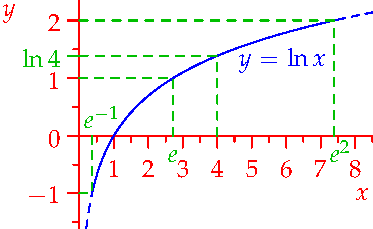
\includegraphics{log}
\end{defn}

Since $\exp$ and $\ln$ are inverse functions, we can solve equations in the usual way: for instance,
\[e^{3x+1}=100 \implies 3x+1=\ln 100\implies x=\frac 13(\ln 100-1) \approx 1.202\]



One of the great advantages of logarithms is that they allow every exponential function to be expressed in terms of the natural exponential: by the exponential laws,
\[a^x=(e^{\ln a})^x=e^{x\ln a}\]
This identity is crucial for interpreting and analyzing natural growth models.
% By the chain rule, we now see that
% \[\diff xa^x=(\ln a)e^{x\ln a}=a^x\ln a\]
% Otherwise said, the solution to the natural growth equation $\diff[y]{x}=(\ln a)y$ is the exponential $y=a^x$.



\begin{example}{}{}
A population of rabbits doubles in size every 6 months. If there are 10 rabbits at the start of the year, how many rabbits do we expect there to be after 9 months, and how rapidly is the population increasing (births/month).\par
\begin{minipage}[t]{0.6\linewidth}\vspace{-3pt}
  We are told that the population of rabbits after $t$ months is
  \[P(t)=10\cdot 2^{t/6}\]
  After 9 months the population will be approximately
  \[P(9)=10\cdot 2^{3/2}=20\sqrt 2\approx 28.28\text{ rabbits}\]
  Moreover,
  \end{minipage}\begin{minipage}[t]{0.4\linewidth}\vspace{-10pt}
  \flushright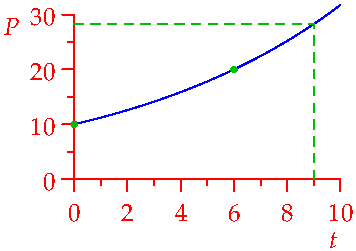
\includegraphics{rabbits}
  \end{minipage}\par\vspace{-3pt}
  \[
  \diff tP(t)=\diff t10e^{\frac t6\ln 2}=\frac{10\ln 2} 62^{t/6}
  \implies P'(9)=\frac{10\ln 2}62^{3/2}\approx 3.27\text{ rabbits/month}
  \]
  If you ask students this question, what do you expect to be the most common \emph{incorrect} answers? Why?
\end{example}

%  mistakes might a student make if they were given the previous example? Why might they obtain the incorrect answer of 25 rabbits?

\goodbreak

\boldsubsubsection{The Logarithm Laws and General Logarithms}


The logarithm laws should be familiar to you; they follow immediately from the above definition and the exponential laws (page \pageref{pg:explaws})
\begin{gather*}
e^{\ln x+\ln y}=e^{\ln x}e^{\ln y}=xy=e^{\ln xy}\implies \tcbhighmath{\ln xy=\ln x+\ln y}\\
\text{Similarly}\quad \tcbhighmath{\ln\tfrac xy=\ln x-\ln y\quad\text{and}\quad \ln x^r=r\ln x}\tag{$\ast$}
\end{gather*}
Amongst other things, these laws allow us to solve more general exponential equations.
\[2^{x}=5\implies x\ln 2=\ln 5\implies x=\frac{\ln 5}{\ln 2}\approx 2.322\]
More generally, if $a>0$ and $a\neq 1$, then the exponential function with base $a$ is invertible:
\[y=f(x)=a^x=e^{x\ln a}\implies \ln y=x\ln a\implies x=\frac{\ln y}{\ln a}\implies f^{-1}(x)=\frac{\ln x}{\ln a}\]

\begin{defn}{}{}
Given $a>0$ and $a\neq 1$, the \emph{logarithm with base $a$} is the function
\[\log_ax :=\frac{\ln x}{\ln a}\]
\end{defn}

As the inverse of the base $a$ exponential function $y=a^x$, the base $a$ logarithm satisfies
\begin{itemize}
	\item If $x>0$, then $a^{\log_a x}=x$;
	\item If $y\in\R$, then $\log_a a^y=y$.
\end{itemize}
The natural logarithm has base $e$. Unless the base is very simple (e.g.{} $a=2$ or 10), we typically stick to using the natural logarithm. On a calculator, the `log' button means $\log_{10}$.
% In part this stems from the original reason for the invention of logarithms: \emph{log tables} which were used to simplify multiplication of large numbers. For example, to multiply $x=8,457$ by $y=29,143$, one would have followed these steps:
% \begin{enumerate}
%   \item Look up the values $\log_{10}x\approx 3.9272$ and $\log_{10}y\approx 4.4645$ in a log table.
%   \item Compute $\log_{10}xy=\log_{10}x+\log_{10}y\approx 8.3917$
%   \item Use the log table for a second time to obtain $xy\approx 10^{8.3917}\approx 246$ million
% \end{enumerate}





\begin{exercises}{}{}
\exstart Find the solution to the equation $4^{2-\sqrt x}=10$.
\begin{enumerate}\setcounter{enumi}{1}
  \item Find the value of $x$ which satisfies the equation $4^{6x}=8$. Your answer should not contain any logarithms\ldots
  %, then $6x=\log_48=\log_44^{3/2}=\frac 32\implies x=\frac 14$

  \item $y=a^x$ satisfies the natural growth equation $\diff[y]x=ky$; what is the value of $k$?
  
	\item Verify the remaining logarithm laws $(\ast)$.
%\[\ln\frac xy=\ln x-\ln y,\qquad \ln x^r=r\ln x\]
  \item By differentiating the expression $e^{\ln x}=x$, verify that $\diff x\ln x=\frac 1x$.
  
  \item Sketch a graph of the functions $f(x)=\log_2x$ and $g(x)=\log_{0.5}x$. How are they related? What happens to the graph of $\log_ax$ as $a$ changes?

  \item Logarithms were originally invented not for calculus but to simplify and multiply large numbers. In the pre-calculator era, it was common for students to carry a book of \emph{log tables} for this purpose. Look up a log table and investigate how to use it.
\end{enumerate}
\end{exercises}


\clearpage


\subsection{Modifying the Natural Growth Model}

In this section we discuss several examples of exponential models motivated by real-world situations. Remember that \emph{modelling} always involves some guesswork and assumptions, which necessarily come with trade-offs: simpler assumptions/models are easier to analyze, but tend to be less accurate. Modelling is always a part of a feedback loop:
\begin{quote}
Data/theory suggest a model whose predictions are tested against real-world data, suggesting changes/improvements to the model.
\end{quote}
% \begin{itemize}\itemsep0pt
%   \item Data and/or theory suggest a mathematical model.
%   \item The model's predictions are compared to real-world data which might suggest changes and improvements to the model.
% \end{itemize}
Applied mathematicians typically desire a `Goldilocks' model which: complicated enough to make accurate predictions without being too complicated to use.

\boldsubsubsection{Newton's Law of Cooling}

A just-poured cup of coffee at \ang{210}F is left outside when the air temperature is \ang{50}F. It seems obvious that the coffee will cool down slowly \emph{towards} \ang{50}F; but how?\smallbreak

To help decide how to model this, ask yourself some questions:

\begin{enumerate}%\itemsep0pt
  \item When should the rate of cooling be most rapid?
  \item What happens to the rate of change in the long run (large time)?
  \item Can you suggest a family of functions which behave in this manner?
\end{enumerate}


Hopefully it seems reasonable to model this with a shifted exponential function, where  the temperature $T(t)$ of the coffee at time $t$ satisfies\par
\begin{minipage}[t]{0.6\linewidth}\vspace{-8pt}
\[T(t)=50+160e^{-kt}\]
for some positive constant $k$. This satisfy all our criteria:
\begin{itemize}%\itemsep0pt
  \item $T(0)=\ang{210}$F.
  \item As $t$ increases, $e^{-kt}$ decreases to zero, so $T(t)$ decreases towards \ang{50}F.
  %\item The rate of cooling $\nm{\diff[T]{t}}=110ke^{-kt}$ is largest at $t=0$ and decreases as $t$ increases. 
\end{itemize}
\end{minipage}\hfill\begin{minipage}[t]{0.39\linewidth}\vspace{-15pt}
\hfill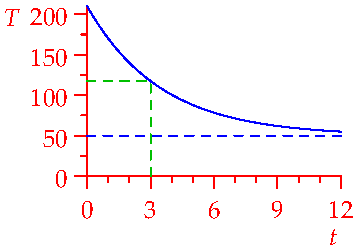
\includegraphics{coffee}
\end{minipage}\par
\begin{itemize}
  \item The rate of cooling $\smash[t]{\nm{\diff[T]{t}}}=160ke^{-kt}$ is largest at $t=0$ and decreases as $t$ increases. 
\end{itemize}

To complete the model, it is enough to supply one further data point.\par

Suppose after 2 minutes that the temperature of the coffee is \ang{140}F. How long does it take for the coffee to cool to \ang{100}F?\smallbreak

We know that $140=T(2)=50+160e^{-2k}$, whence
\[e^{-2k}=\frac{140-50}{160}=\frac 9{16}\implies e^{-k}=\frac 34\implies T(t)=50+160\left(\frac 34\right)^t\]
When $T(t)=100$, we see that
\[\left(\frac 34\right)^t=\frac{100-50}{160}=\frac 5{16}\implies t=\frac{\ln\frac 5{16}}{\ln\frac 34} =\frac{\ln 16-\ln 5}{\ln 4-\ln 3}\approx 4.043\text{ minutes}\]


\goodbreak

This is an example of a general model called \emph{Newton's law of cooling,} which asserts that the rate of temperature change of a body is proportional to the \emph{difference} between the body and its surroundings. We have a simple modification of Theorem \ref{thm:natgrowth}

\begin{cor}{}{newtoncool}
If $M$ and $k$ are constant, then
\[\diff[y]{t}=k(M-y)\iff y(t)=M+(y_0-M)e^{-kt}\]
where $y_0=y(0)$ is the initial value.
\end{cor}



\boldsubsubsection{The Logistic Model}

The natural growth model has one enormous drawback when applied to real-world populations: if $k>0$, then a function $y(t)=y_0e^{kt}$ \emph{grows unboundedly}! In typical situations, environmental limitations (availability of food, water, space) mean that populations do not \emph{explode} like this. The \emph{logistic model} attempts to describe this phenomenon; it is based on two assumptions:\par
\begin{minipage}[t]{0.6\linewidth}\vspace{-5pt}
\begin{itemize}
  \item When a population $y$ is small, we want it to grow naturally $\diff[y]{t}\propto y$.
	\item We want $y$ to approach a positive value $M$ as $t\to \infty$.
\end{itemize}
Given constants $k,M>0$, the \emph{logistic differential equation}
\[\tcbhighmath{\diff[y]{t}=ky(M-y)}\]
\end{minipage}\hfill
\begin{minipage}[t]{0.39\linewidth}\vspace{0pt}
\flushright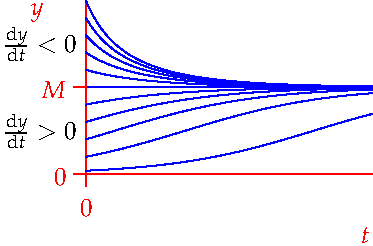
\includegraphics{logisticsf}
\end{minipage}\medbreak
accomplishes both requirements. $M$ is often referred to as the \emph{carrying capacity} of the environment.



\begin{thm}{}{}
If $y_0=y(0)$, then the solution to the logistic differential equation is
\[y(t)=\frac{y_0M}{y_0+(M-y_0)e^{-kMt}}\]
\end{thm}

You can check directly that this satisfies the differential equation just by differentiating, though it's a little ugly. If you've studied differential equations the method of separation of variables supplies the converse.

\begin{example}{}{wort}
A brewer pitches 100 billion yeast cells into a starter wort with the goal of growing it to 200 billion cells. After one hour, the wort contains 110 billion cells.
\begin{enumeratea}
  \item How long must the brewer wait if we use a natural growth model?
  \item How long must the brewer wait if we use a logistic model where we also assume that the wort contains enough sugar to grow 250 billion yeast cells?
  %\item For both models, what is the maximum growth rate and at what time does it occur?
\end{enumeratea}

Let $P(t)$ be the yeast population in billions at time $t$ hours. We therefore have $P(0)=100$ and $P(1)=110$, and want to find $t$ such that $P(t)=200$.
\begin{enumeratea}
  \begin{minipage}[t]{0.6\linewidth}\vspace{0pt}
  \item The model is $\diff[P]{t}=ky$, which has solution
  \[P(t)=P_0e^{kt}=100e^{kt}\]
  Evaluating at $t=1$ yields $1.1=e^k$ whence
  \[P(t)=100(1.1)^t\implies t=\frac{\ln(0.01 P)}{\ln 1.1}\approx 7.27\,\text{hours}\]
	\item The model is $\diff[P]{t}=ky(250-y)$, with solution
	\[P(t)=\frac{25000}{100+(250-100)e^{-250kt}} =\frac{500}{2+3e^{-250kt}}\]
  \end{minipage}\begin{minipage}[t]{0.4\linewidth}\vspace{0pt}
  \flushright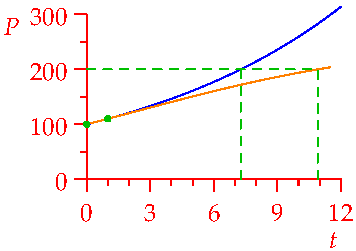
\includegraphics{wort}
  \end{minipage}\smallbreak
  
	Evaluating at $t=1$ yields
	\[110=\frac{500}{2+3e^{-250k}} \implies e^{250k}=\frac{33}{28}\]
	whence
	\[P(t)=\frac{500}{2+3\left(\frac{28}{33}
	\right)^t} \implies t=\frac{\ln 6}{\ln\frac{33}{28}} \approx 10.91\,\text{hours}\]
  \end{enumeratea}
\end{example}


The logistic model is easily generalized.

\begin{example}{}{fish}
The population $P(t)$ (in 1000s) of fish in a lake obeys the logistic equation
\begin{minipage}[t]{0.6\linewidth}\vspace{-10pt}
\[\diff[P]{t}=\frac 1{16}P(10-P)\]
where $t$ is measured in months. The first graph shows how the population recovers over a year if it starts at 2500 fish.\smallbreak
Now suppose 1000 fish are `harvested' from the lake each month. The new model is then
\begin{align*}
\diff[P]{t}&=\frac 1{16}P(10-P)-1=-\frac 1{16}(P^2-10P+16)\\
&=-\frac 1{16}(P-2)(P-8)
\end{align*}
Substituting $Q=P-2$, this is again logistic!
\[\diff[Q]{t}=\frac 1{16}Q(6-Q)\]
\end{minipage}\hfill\begin{minipage}[t]{0.39\linewidth}\vspace{0pt}
\flushright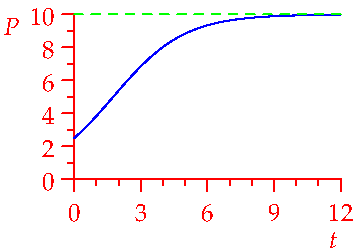
\includegraphics{fish}\par
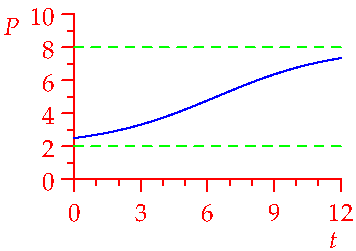
\includegraphics{fish2}
\end{minipage}
Provided the initial population $P(0)=Q(0)+2$ is greater than 2000 fish, we expect the population to eventually stabilize at 8000 fish, though it takes a long time to get close to this if we start, as in the second graph, with only a little over 2000 fish.
\end{example}
\goodbreak



\boldsubsubsection{Public-health Interventions}\phantomsection\label{pg:virus}

A population of 10,000 people is exposed to a novel virus. The best scientific understanding is that 1\% of the susceptible population per day contracts the virus, the effects of the illness last ten days, after which a patient recovers and is immune from reinfection.
\begin{enumerate}
  \item Model the evolution of the sick and immune populations over the next 120 days.\smallbreak
  Let $u(t)$, $s(t)$ and $i(t)$ represent the uninfected, sick and immune populations on day $t$. Then
\[u(t+1)= 0.99u(t),\quad u(0)=10000\implies u(t)=10000\cdot 0.99^t\]
The sick population is the sum of the previous 10 days' decrease in the at risk population:
\[s(t)=\begin{cases}
u(0)-u(t)=10000(1-0.99^t)&\text{if }t\le 10\\
u(t-10)-u(t)=10000(0.99^{-10}-1)0.99^t=1057\cdot 0.99^t&\text{if }t> 10
\end{cases}\]
The immune population is the difference between these and the total population
\[i(t)=10000-u(t)-s(t)=\begin{cases}
0&\text{if }t\le 10\\
10000-11057\cdot 0.99^t&\text{if }t> 10
\end{cases}\]
After 120 days, we have
\[u(120)=2994,\qquad s(120)=316,\qquad i(120)=6690\]
  
  \item Suppose 6000 vaccines are available. Discuss how these should be deployed. What should the goal be? Discuss the following strategies; for simplicity, assume the vaccines are 100\% effective and work instantly.
  \begin{enumerate}
    \item[\textcolor{red}{(a)}] Use all vaccine doses immediately.
  	\item[\textcolor{Goldenrod}{(b)}] Wait 30 days until some people are immune, then use all vaccines on the uninfected population.
  	\item[\textcolor{Green}{(c)}] Vaccinate 100 uninfected people per day.
  	\item[(d)] Wait until there are 6000 uninfected people remaining, then vaccinate them all at once.
	\end{enumerate}
\end{enumerate}
It is much easier to analyze this problem using a \href{http://math.uci.edu/~ndonalds/math8/virus.xlsx}{spreadsheet,} though we can also do things analytically. Here are graphs of what happens under a \textcolor{blue}{non-intervention scenario} and the first three vaccination campaigns.
\begin{center}
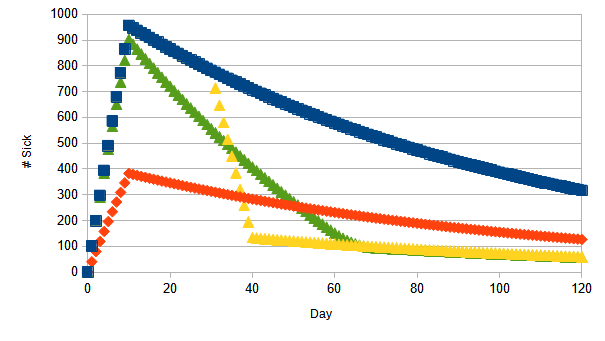
\includegraphics[scale=0.69]{vax-new}
\end{center}

\goodbreak


\begin{exercises}
\exstart A cup of coffee is left outside on a warm day when the surrounding temperature is \ang{90}F. Suppose the initial temperature of the coffee is \ang{200}F and that its temperature after 2 minutes is \ang{170}F. Find the temperature as a function of time.

\begin{enumerate}\setcounter{enumi}{1}
  \item Consider Corollary \ref{cor:newtoncool}.
	\begin{enumerate}
	  \item Check that $y(x)=M+(y_0-M)e^{-kt}$ satisfies the differential equation.
	  \item A student believes that Theorem \ref{thm:natgrowth} is true. How would you convince them, \emph{in the simplest possible way,} that the \emph{only} solution to $y'=k(M-y)$ is as given in part (a)?
	\end{enumerate}

% 	\item A body with initial temperature $T_0$ is placed in an environment with constant temperature $M<T_0$. Suppose that the temperature $T(t)$ obeys Newton's law of cooling, and that it takes $t_1$ seconds for the body to cool to $\frac{T_0+M}2$. Find the temperature at time $t$ and determine how long it takes for the body to cool to $\frac 13(T_0+2M)$.
	
	\item For both models in Example \ref{ex:wort}, what is the maximum growth rate of the yeast population, and at what time does it occur?
	

	\item In Example \ref{ex:fish}, if the initial population is 3000 fish and 1000 fish are harvested per month, how long does it take for the population to recover to 6000 fish?
	
	
  \item Plutonium-238 has a \emph{half-life} of 88 years, meaning that after 88 years half of the isotope has decayed to another element (in this case uranium-234).
  \begin{enumerate}
  	\item If you start with 100 grams of plutonium, find a model for how much remains after $t$ years.
  	\item How long will take for the mass to decay to 10 grams, and at what rate will it be decaying? 
  \end{enumerate}
  
	
	\item\begin{enumerate}
	  \item If public health officials wanted to eradicate the virus on page \pageref{pg:virus} completely by using all vaccine doses on one day, on which day should they act?
	  \item Find the number of uninfected people as a function of time under the 100 per day for 60 days vaccination scenario.
	\end{enumerate}
\end{enumerate}
\end{exercises}
